\documentclass[review]{elsarticle}

\usepackage{lineno,hyperref}
\modulolinenumbers[5]
\usepackage[table,xcdraw]{xcolor}
\usepackage{csquotes}
\usepackage{graphicx}
\usepackage{cleveref}
\usepackage{paralist}
\usepackage{listings}
\usepackage[T1]{fontenc}
\usepackage{pdflscape}
\usepackage{afterpage}
\biboptions{numbers,sort&compress}


\crefname{listing}{\lstlistingname}{\lstlistingname}
\Crefname{listing}{Listing}{Listings}

\journal{Computer Science Review}

%%%%%%%%%%%%%%%%%%%%%%%
%% Elsevier bibliography styles
%%%%%%%%%%%%%%%%%%%%%%%
%% To change the style, put a % in front of the second line of the current style and
%% remove the % from the second line of the style you would like to use.
%%%%%%%%%%%%%%%%%%%%%%%

%% Numbered
%\bibliographystyle{model1-num-names}

%% Numbered without titles
%\bibliographystyle{model1a-num-names}

%% Harvard
%\bibliographystyle{model2-names.bst}\biboptions{authoryear}

%% Vancouver numbered
%\usepackage{numcompress}\bibliographystyle{model3-num-names}

%% Vancouver name/year
%\usepackage{numcompress}\bibliographystyle{model4-names}\biboptions{authoryear}

%% APA style
%\bibliographystyle{model5-names}\biboptions{authoryear}

%% AMA style
%\usepackage{numcompress}\bibliographystyle{model6-num-names}

%% `Elsevier LaTeX' style
\bibliographystyle{elsarticle-num}
%%%%%%%%%%%%%%%%%%%%%%%

\begin{document}

\begin{frontmatter}

\title{Cross-chain Smart Contract Invocations -- a Multi-vocal Literature Review Protocol\\V1.0}
\author[iaas]{Ghareeb Falazi\corref{corrauthor}}
\author[iaas]{Uwe Breitenb\"ucher}
\author[iaas]{Frank Leymann}
\author[tuhh]{Stefan Schulte}
\address[iaas]{Institute of Architecture of Application Systems, University of Stuttgart\\Universit\"atsstra\ss{}e 38, 70569 Stuttgart}
\address[tuhh]{Institute of Data Engineering, Hamburg University of Technology\\Am Schwarzenberg-Campus 3, 21073 Hamburg}
\cortext[corrauthor]{Corresponding author}
\ead{ghareeb.falazi@iaas.uni-stuttgart.de}


\begin{abstract}
This document introduces the protocol that describes how a planned Multi-vocal Literature Review (MLR) regarding Cross-chain Smart Contract Invocation (CCSCI) is going to be conducted.
The main purpose of having this protocol is to avoid bias when selecting primary sources and processing them.
Furthermore, it helps potential co-authors gain an overview of the topic, which helps them to decide whether to participate or not.
\end{abstract}

%\begin{keyword}
%\texttt{elsarticle.cls}\sep \LaTeX\sep Elsevier \sep template
%\MSC[2010] 00-01\sep  99-00
%\end{keyword}

\end{frontmatter}

\tableofcontents

\linenumbers

\section{Introduction and Background}
\label{sec:introduction-and-background}
In the past few years, blockchains have expanded their applicability to domains beyond finance and cryptocurrencies, such as health care management~\cite{Tuli2020Healthcare}, supply chains management~\cite{Montecchi2019SupplyChains}, identity management~\cite{Zhu2018IdentityManagement}, smart grids~\cite{Pop2018SmartGrid}, and others.
However, blockchains suffer from issues that complicate their mass adoption and integration into enterprise systems.
One of these issues is the lack of \emph{blockchain interoperability}.
An \emph{interoperable blockchain architecture} is defined as \enquote{(...) a composition of distinguishable blockchain systems, each representing a unique distributed data ledger, where atomic transaction execution may span multiple heterogeneous blockchain systems, and where data recorded in one blockchain is reachable, verifiable and referenceable by another possibly foreign transaction in a semantically compatible manner}~\cite{Hardjon2020Interoperability}.

\begin{figure}
	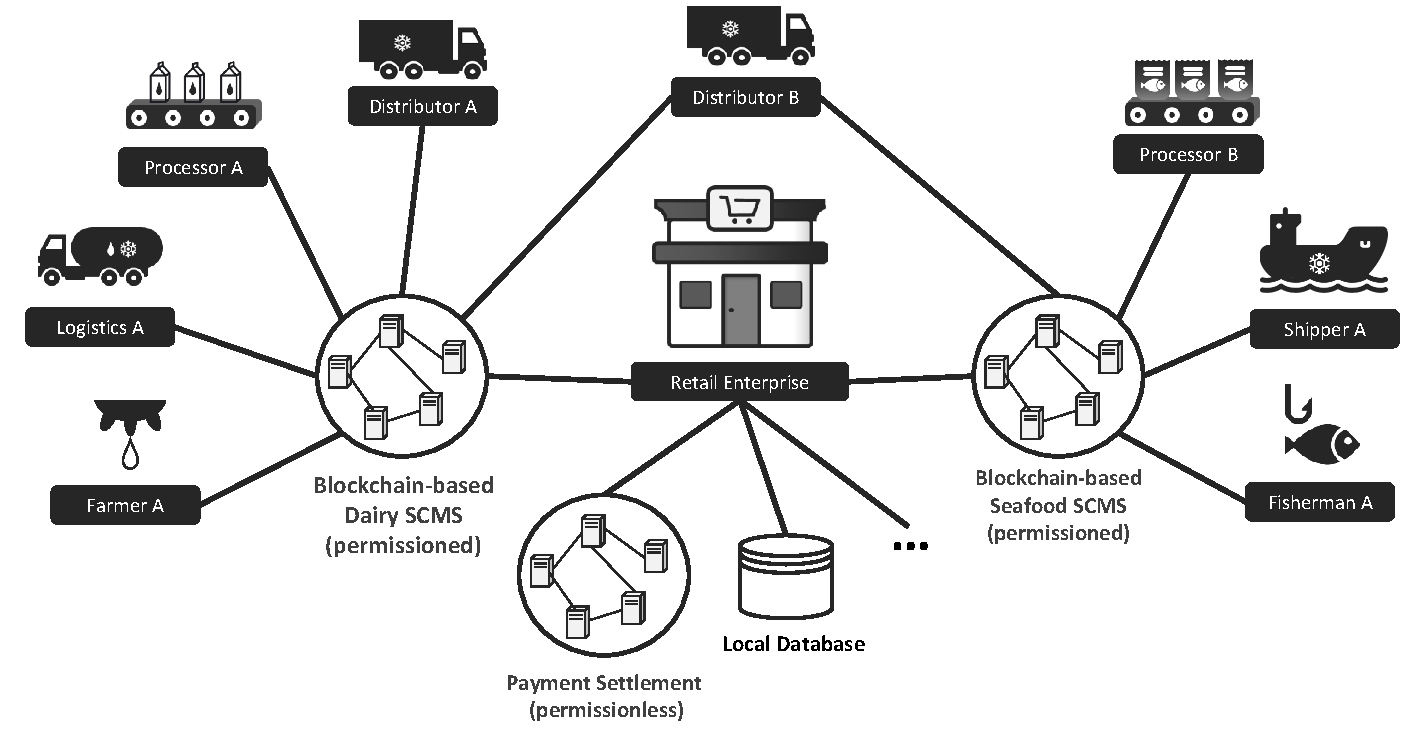
\includegraphics[width=\linewidth]{graphics/scenario}
	\caption[Running example]{Running example of an enterprise connected to multiple permissioned and permissionless blockchain systems as well as other transactional resources.}
	\label{fig:scenario}
\end{figure}

A prominent reason why blockchain interoperability is relevant in the domain of enterprise integration is that enterprises may need to communicate with multiple blockchain systems simultaneously in real-world settings.
However, due to the vast heterogeneity of available blockchain systems, the lack of blockchain standardization, as well as certain properties unique to blockchains, an enterprise wishing to perform such an integration will face a non-trivial task~\cite{Falazi2020_UnifiedIntegrationBlockchains}.
To demonstrate this problem, \Cref{fig:scenario} shows two simplified supply chains for seafood and dairy products.
The dairy products supply chain starts from cattle ranches (Farmer A), which produce milk that is transported daily to processing facilities (Processor A) with the help of logistics partners (Logistics A).
Finally, distributors (Distributor A and Distributor B) transport the resulting milk cartons to retailers (Retail Enterprise).
The seafood supply chain proceeds similarly starting from individual fishermen (Fisherman A), or commercial fisheries, which catch seafood resources like fish.
Next, fish are transported via shipping firms (Shipper A) to their first buyers overseas (Processor B), which process and package them appropriately.
Finally, the packaged fish are transported to retailers (Retail Enterprise) via domestic distributors (Distributor B).

We assume that the participants of each supply chain agree on using a blockchain to manage their transactions and to store the state of the various products.
The goal is to facilitate end-to-end product provenance and to cut down on costs that otherwise would be spent on third-party intermediaries.
To this end, a \emph{permissioned blockchain}, such as Hyperledger Fabric~\cite{Androulaki2018Fabric} ensures confidentiality, transaction durability, and acceptable performance, since access to blockchain data is limited to registered users, and the used consensus mechanism is usually a form of Byzantine Fault Tolerant (BFT) protocols that provide transaction finality and better throughput~\cite{cachin2017consensus}.
Moreover, the agreed-upon collaboration logic is implemented in the form of one or more \emph{smart contracts}~\cite{wood2021ethereum} and deployed on the blockchain.
Due to overwhelming overhead, scalability issues, and low interest, it is, however, unrealistic to assume that the participants of all possible supply chains agree on the same blockchain platform.
This means that multiple blockchain instances will likely coexist to support different supply chains, e.g., for the seafood and milk processing sectors (this might even apply within the same supply chain).
Furthermore, since many blockchain technologies exist with different trade-offs and guarantees~\cite{Falazi2019_TransactionalPropertiesBlockchains}, it is also not possible to assume that all considered blockchain instances are of the same technology.
In this example, we assume that the seafood supply chain is managed by a  private deployment of the Ethereum blockchain running the Proof-of-Authority (PoA) consensus mechanism~\cite{Szilagyi2017Clique}, whereas the dairy product supply chain is managed by a deployment of the Hyperledger Fabric permissioned blockchain~\cite{Androulaki2018Fabric}. 

Due to this heterogeneity, and as we indicated before, substantial integration challenges arise when certain participants, like the (Retail Enterprise) and (Distributor B), are involved in both, and potentially more, supply chains at the same time.
Things get even more complicated when further blockchains are used for other purposes like payment settlement.
These challenges take many forms.
In this work, we study the challenge of realizing a subset of Cross-chain Business Transactions (CCBT)\footnote{We use the terms \enquote{Cross-chain}, \enquote{Cross-blockchain}, and \enquote{Cross-ledger} interchangeably.}.
CCBT, in general, are business transactions that involve resources (cryptocurrencies, tokens, arbitrary data, or smart contracts) of more than one blockchain, or that involve other transactional resources, like databases or message queues, in addition to blockchains.
Although the execution of operations on resources is atomic within the boundaries of a single system~\cite{Tai2017SALT}, CCBTs are not easy to realize in an atomic manner and are subject to extensive research~\cite{Qasse2019,Zakhary2019TransactionalSmartContracts,Siris2019,Zamyatin2019SoKCA,Borkowski2019}.
A subcategory of CCBTs addresses Cross-chain Smart Contract Invocations (CCSCI).
In this case, a blockchain-external client application executes a transactional program that includes invocations to multiple smart contract functions of different, possibly heterogeneous, blockchains.
The invocation can also involve other transactional resources like database management systems.
This is mostly relevant for enterprise integration scenarios.
For example, if a customer shopping at one of the shops of the (Retail Enterprise) of \Cref{fig:scenario} buys a milk carton and a bag of frozen fish together, this will cause the software system of the (Retail Enterprise) to trigger a CCSCI.
The CCSCI will execute a smart contract function in the Blockchain-based Dairy Supply-chain Management System (SCMS) that will change the status of the milk carton, and a smart contract function in the Blockchain-based Seafood SCMS that will do the same with the fish bag.
It will also update the corresponding entries in the local database, and charge the customer for the purchase.
In addition to the fact that such invocations are hard to execute atomically, the problem remains open on what kind of semantics they have and how to model them in the first place.

Therefore, the planned study aims at uncovering and summarizing how academia and industry have addressed the topic of CCSCIs and discovering the major research gaps left by the current approaches.
To this end, we plan to conduct a Multi-vocal Literature Review (MLR) that includes both peer-reviewed Formal Literature (FL) and high-quality Gray Literature (GL).
To be more precise, in this work we consider the following definitions for formal literature and gray literature:
\begin{description}
	\item[Formal Literature (FL):] any kind of publications that describes a primary study and whose quality is ensured either via a single-blind or a double-blind peer review, such as journal articles or conference proceedings.
	
	\item[Gray Literature (GL):] any kind of publication that describes a primary study or a part thereof and whose quality is not ensured via a single-blind or a double-blind peer review, such as book chapters, technical reports, white papers, software system documentations, blog posts, or even certain videos.
\end{description}


\paragraph{Why to Include Gray Literature?}
Following the recommendations by Garousi et al.~\cite{Garousi2017MLR}, we decided to incorporate gray literature in this study for two notable reasons:
\begin{inparaenum}[(i)]
	\item after considering related surveys (see \Cref{sec:related-work}), we have established that a large volume of work done on blockchains in general and more specifically on the topic of blockchain interoperability is not published in peer-reviewed outlets, like scientific conferences or journals, but rather published in the form of white papers, Web Sites, and blog posts.
	Excluding gray literature will greatly impact the coverage and usefulness of this study.
	\item The relatively large volume of practitioner sources indicate high interest in the topic within the software industry community.
	This community will benefit from synthesizing the insights and evidence of practitioner and academic sources.	
\end{inparaenum}


\section{Overview of the Research Method}
\label{sec:overview-of-the-process}

\begin{figure}
	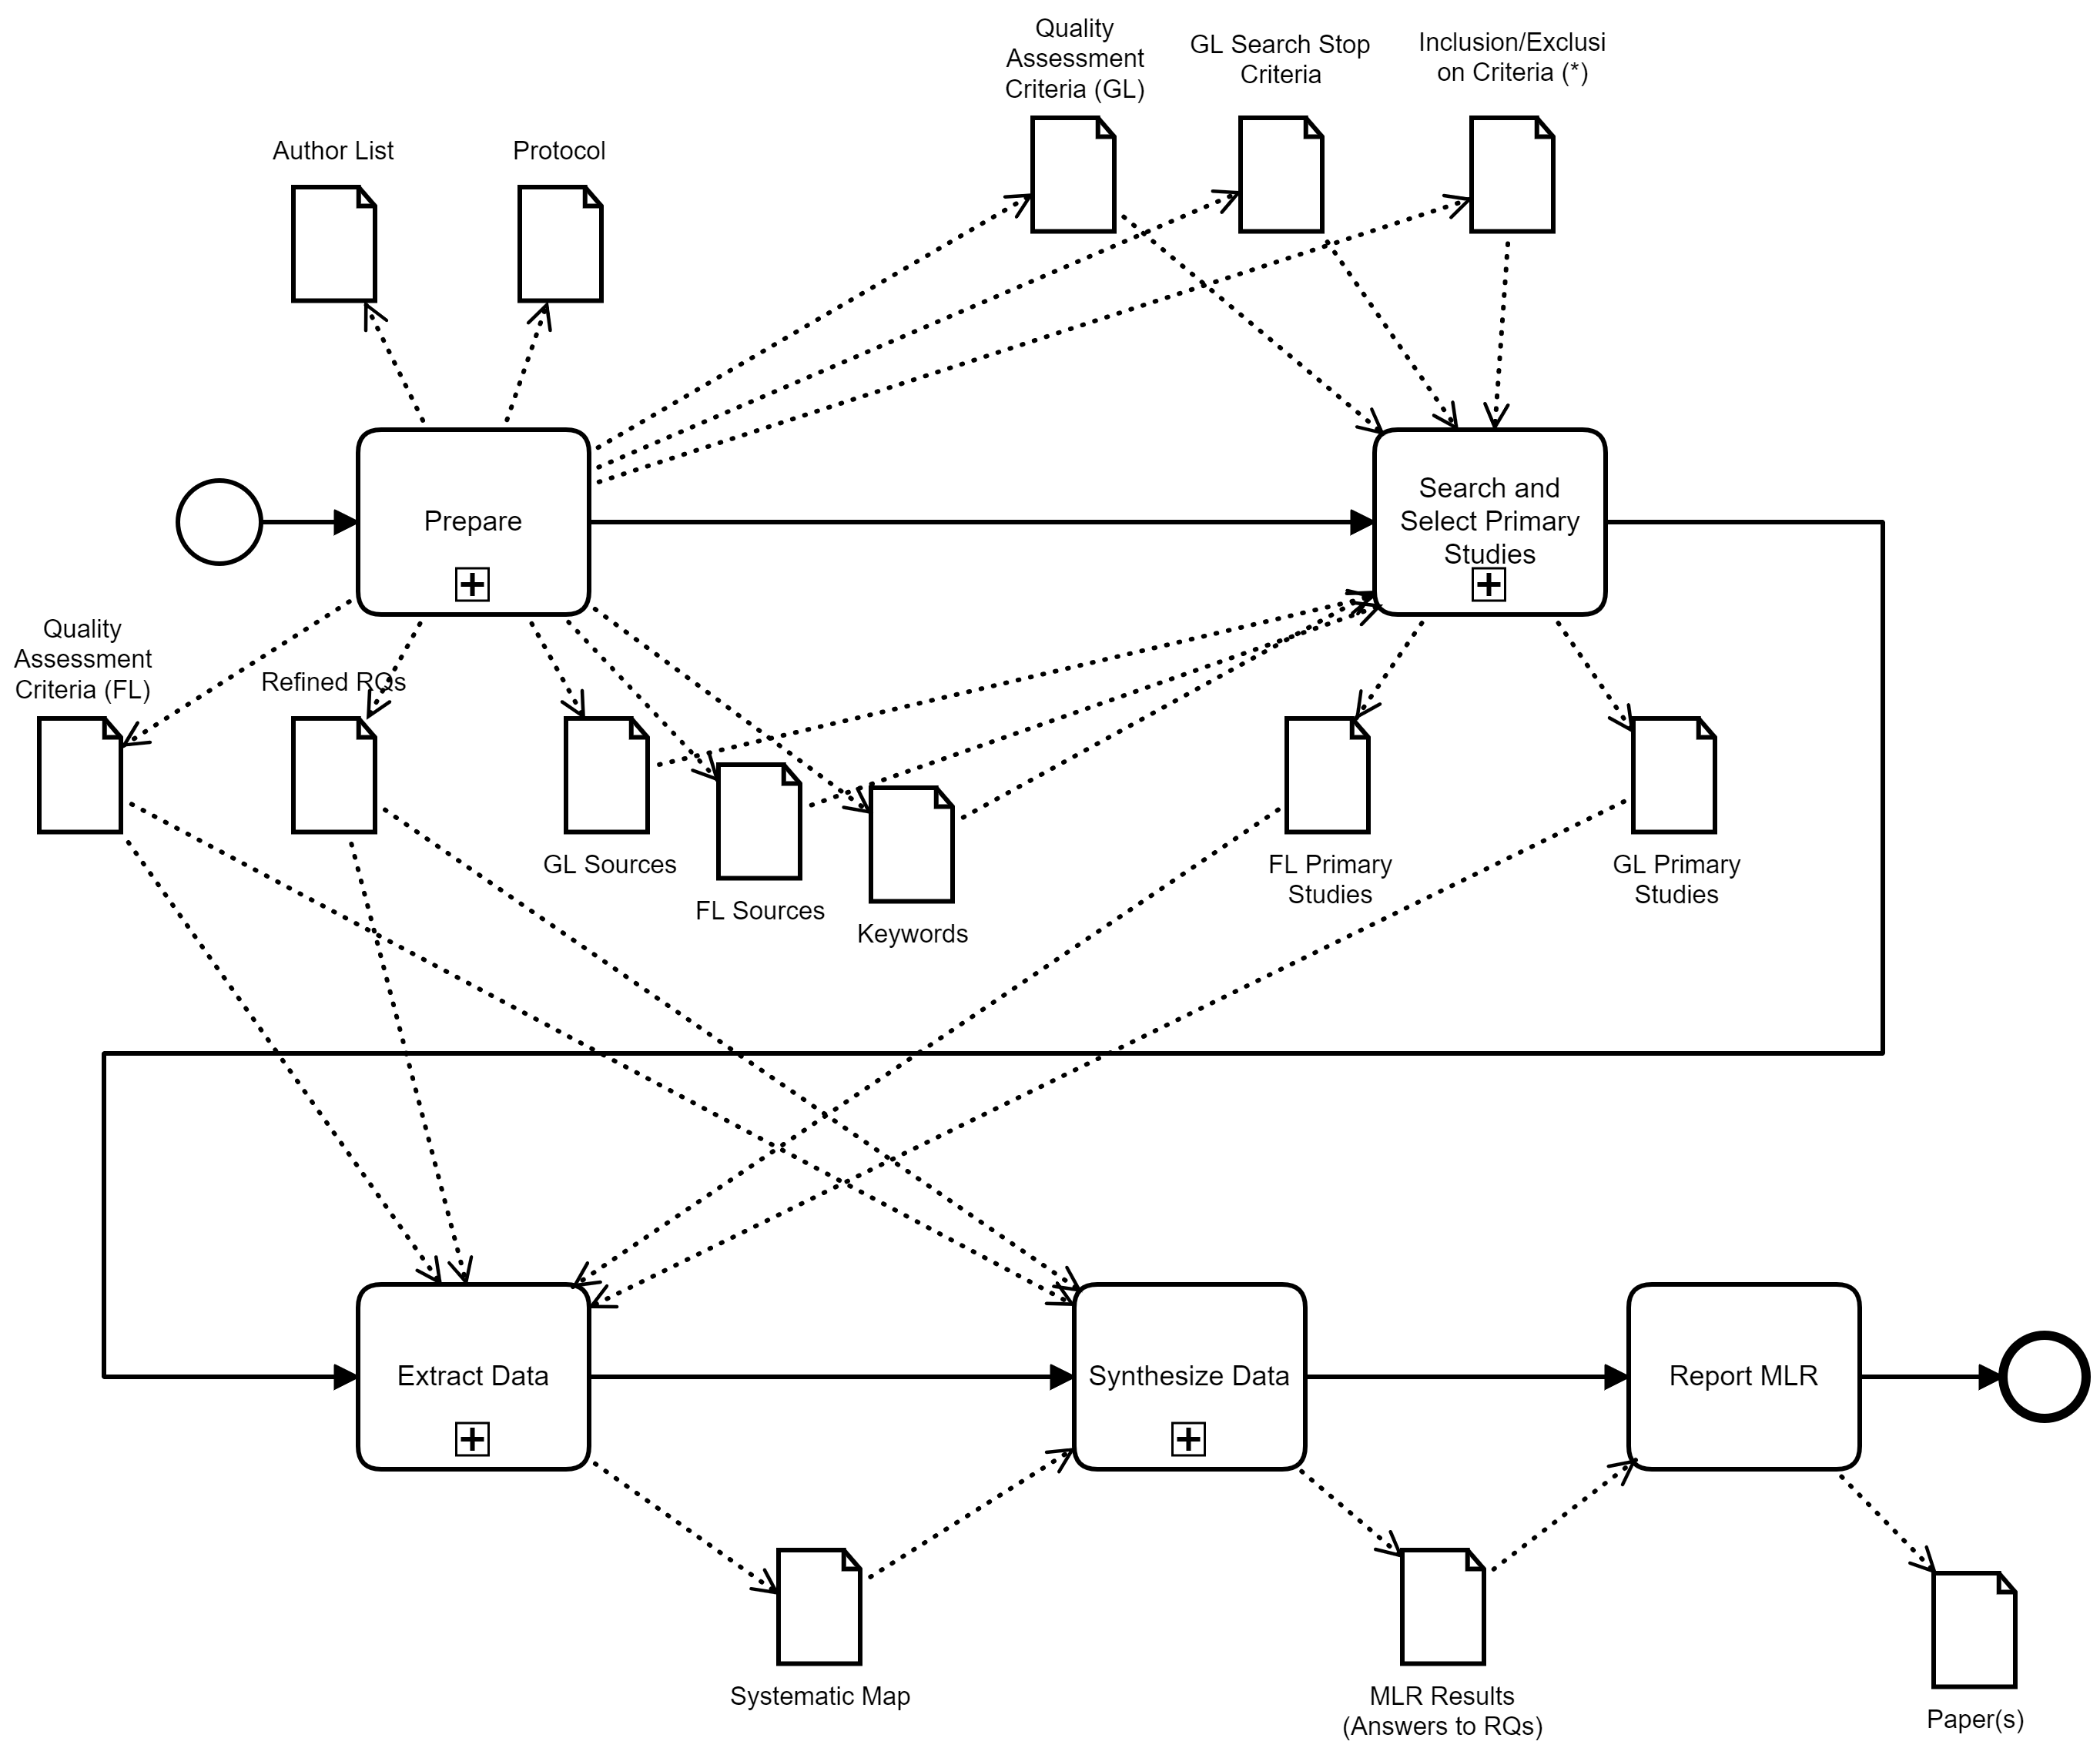
\includegraphics[width=\linewidth]{graphics/process}
	\caption[The MLR process]{The overall process of conducting the MLR.}
	\label{fig:process}
\end{figure}

Following the recommendations by Kitchenham et al.~\cite{Kitchenham2007SLR} and Garousi et al.~\cite{Garousi2017MLR}, we designed a process that defines how this MLR will be conducted.
\Cref{fig:process} shows an overview of this process in the form of a BPMN model.
The process consists of the following major activities, which we explain in terms of the outcomes expected from them (depicted as data objects):
\begin{description}
	\item[Prepare] In this activity, preparatory steps are conducted, which will result in 
	\begin{inparaenum}[(i)]
		\item the specific set of \emph{Research Questions (RQs)} that this MLR will try to answer,
		\item the set of \emph{formal literature sources}, and \emph{gray literature sources} that we will use to search for primary studies,
		\item the set of \emph{keywords} inferred from the RQs and used to search for relevant primary studies in the chosen sources,
		\item the set of \emph{inclusion and exclusion criteria} that will be used to determine whether to include any given primary study in the final list of studies to be thoroughly analyzed or not,
		\item the set of \emph{quality assessment criteria} to be used to assess the quality of the selected GL and FL studies,
		\item the set of \emph{search stopping criteria} for GL studies, which are necessary since it is generally very difficult to have a coverage of 100\% of GL studies~\cite{Garousi2017MLR}, and 
		\item other outputs, like this protocol and the full list of co-authors.
		The detailed steps conducted in this activity are described in \Cref{fig:prepare-detailed}.
	\end{inparaenum}
	\item[Search and Select Primary Study] In this activity, we search for relevant primary studies and select them, which results in the \emph{final list of primary studies} to be analyzed.
	The detailed steps that will be conducted in this activity are explained in \Cref{sec:study-quality-assessment,sec:study-selection-procedure,sec:study-selection-criteria,sec:search-strategy}.
	\item[Extract Data] In this step, we extract the data that will help us answer the RQs from every study in the final list of primary studies.
	The primary outcome of this step is a \emph{systematic map}~\cite{Kitchenham2007SLR}.
	\item[Synthesize Data] In this activity, results extracted from all considered primary studies are synthesized in a coherent set of findings that are able to give clear \emph{answers to the RQs}.
	These answers are the primary outcomes of this activity.
	\item[Report MLR] In this activity, the MLR intermediary and final outcomes are formulated in ways that can be reported to the academic world, as well as practitioners.
	Such reports could take the form of conference or journal papers, magazine articles, presentations, and blog posts to give some examples.
\end{description}

\afterpage{%
	\begin{landscape}
		\begin{figure}
			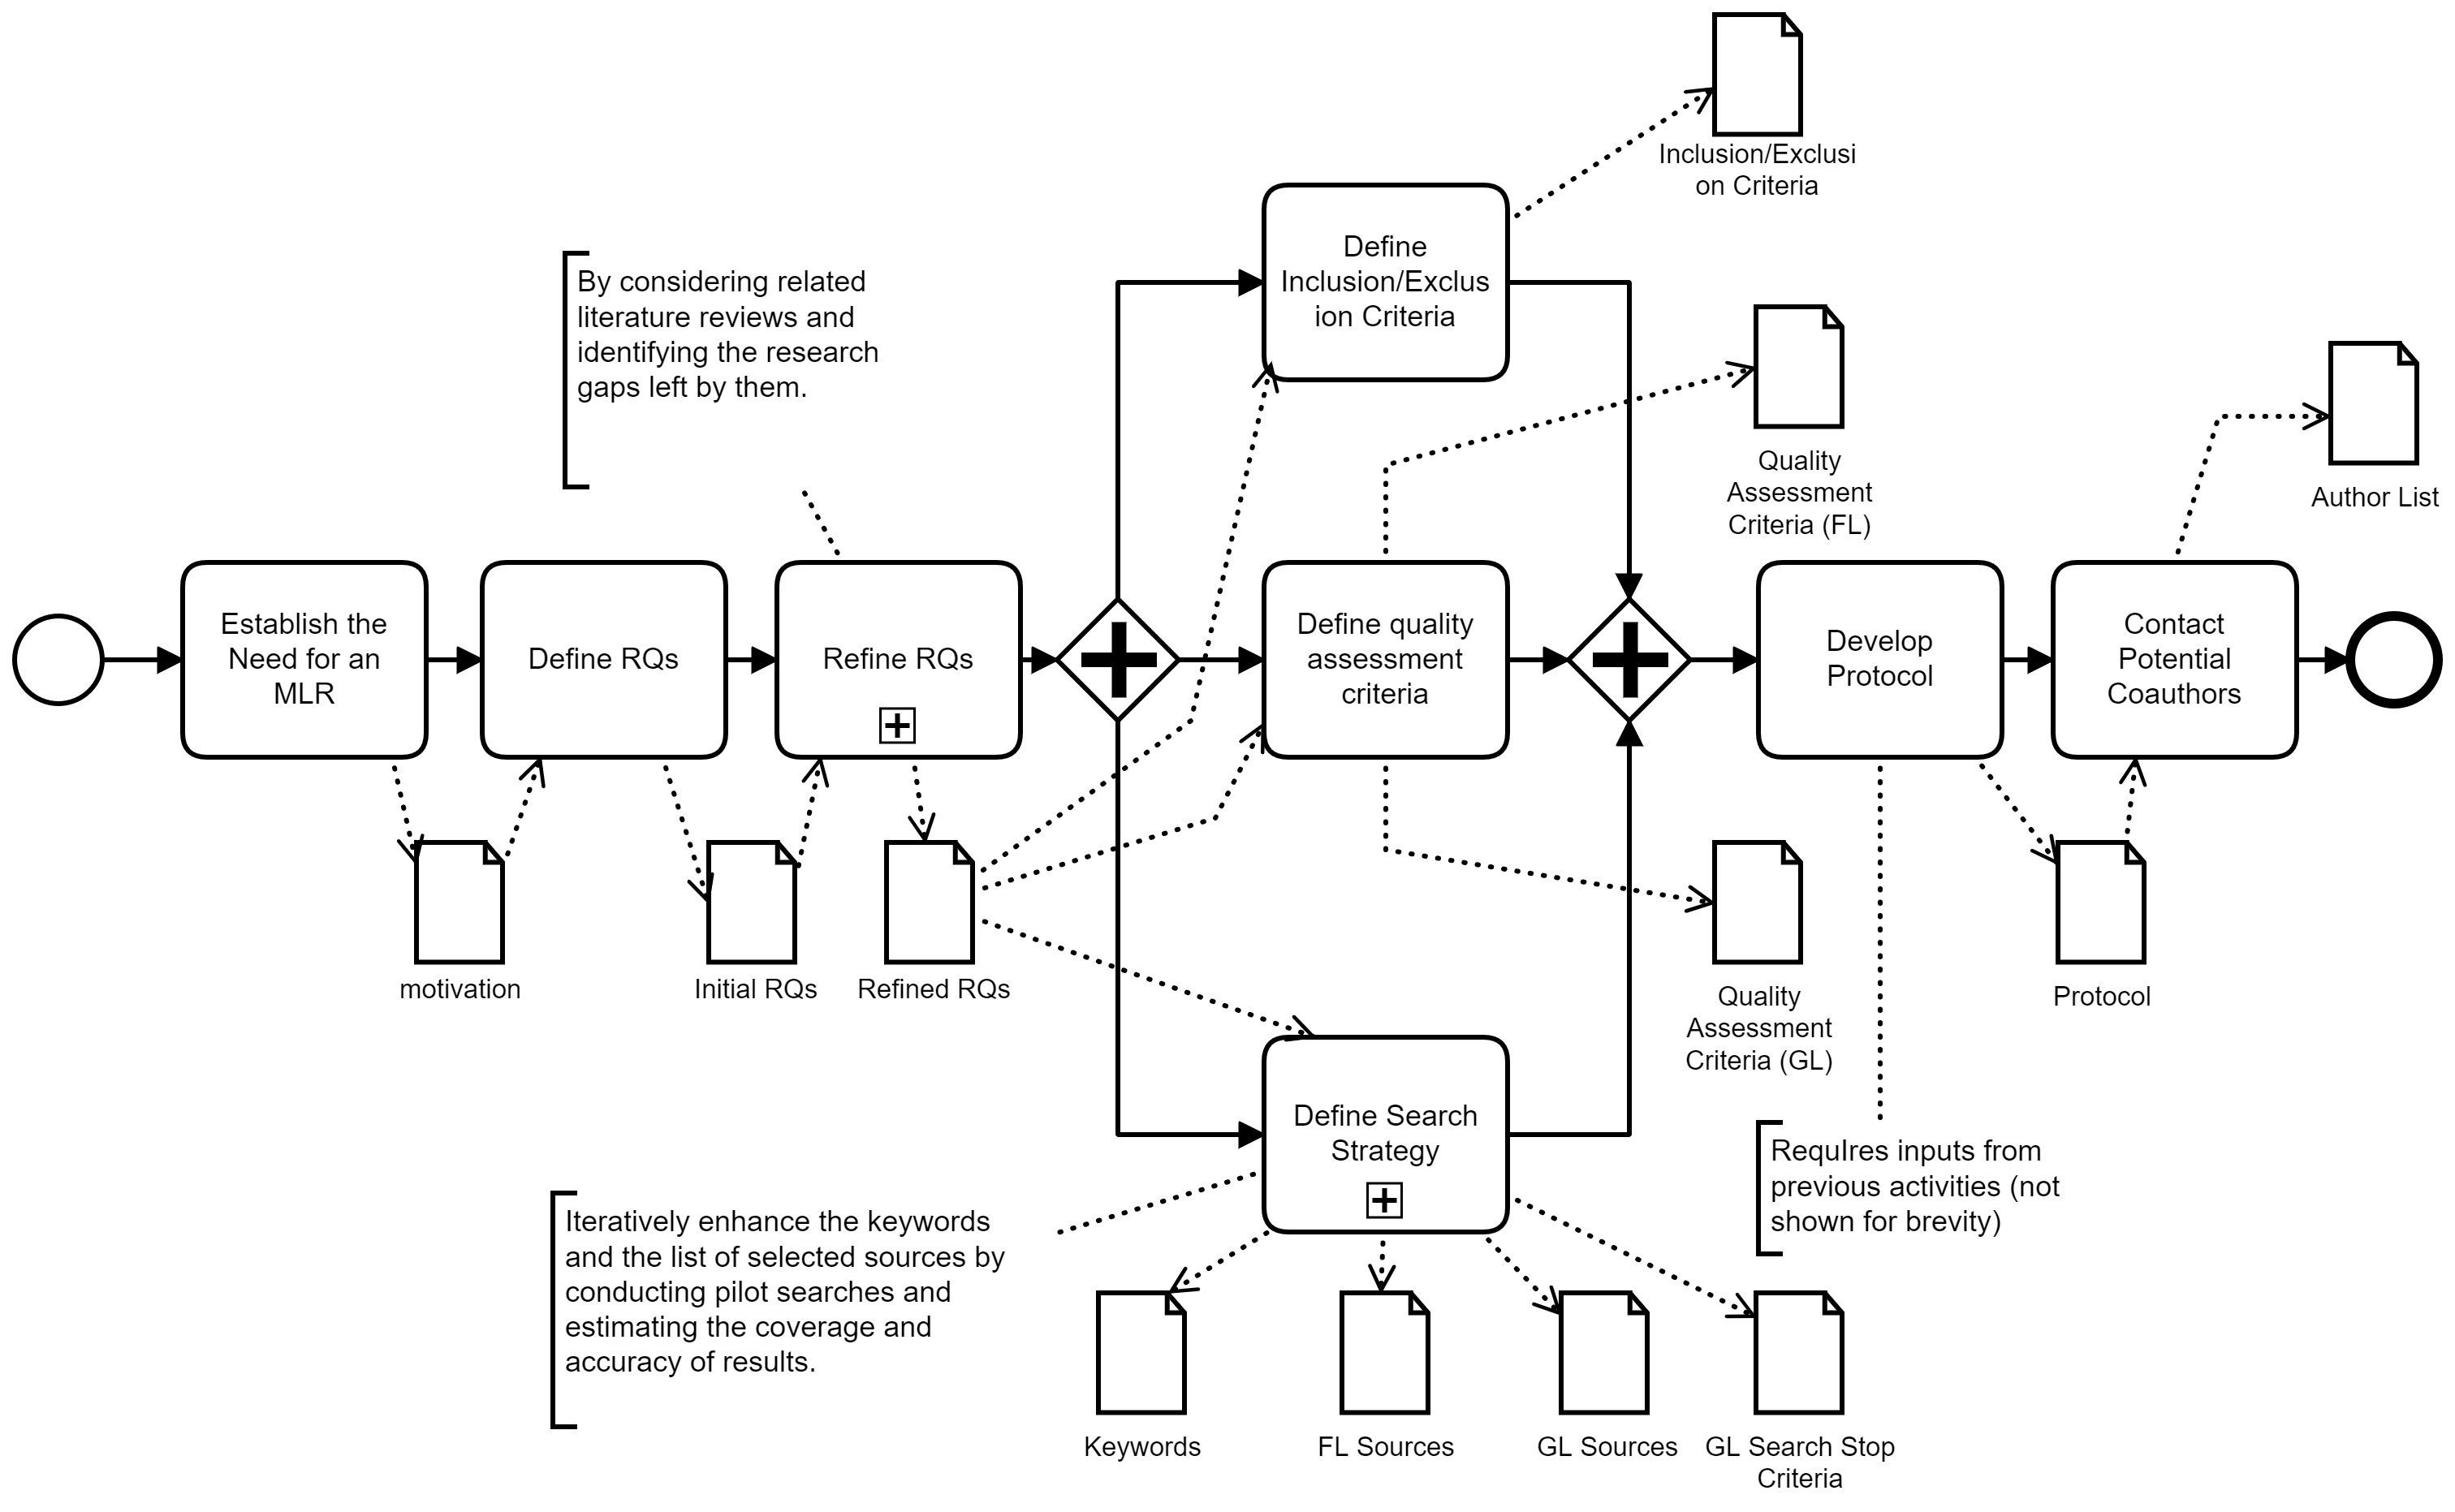
\includegraphics[width=\linewidth]{graphics/planning-overview}
			\caption[Planning overview]{A detailed view of the steps to be taken during the planning activity of the MLR.}
			\label{fig:prepare-detailed}
		\end{figure}
	\end{landscape}
}

\section{Related Work}
\label{sec:related-work}

To have an overview of the topic of blockchain integration and to identify the gaps in the current state-of-the-art, we conducted a mini-literature review that involved related literature reviews.
To conduct this mini-review, we used Google Scholar so that both peer-reviewed reviews as well as reviews published as white papers can be found.
To ease the processing of search results, we used the software \textit{Publish or Perish}\footnote{\url{https://harzing.com/resources/publish-or-perish}}.
We limited the search to the years 2016-2021 since we only wanted recent reviews to be included.
We required the title of search elements to satisfy the following query\footnote{In search queries, "\texttt{?}" is a wildcard denoting any character (including whitespaces).}:
\begin{lstlisting}
	survey | review | sok | state?of?the?art
\end{lstlisting}

In addition, we required the following query to be fulfilled by any part of every search result (title, abstract, body if available, keywords, etc.):
\begin{lstlisting}[caption={The query term used to search for primary and secondary studies.},label={lst:query-string}]
	("inter?blockchain" | "cross?blockchain" | 
	"multi?blockchain" | "inter?chain" | "cross?chain" |
	"multi?chain" | "cross?ledger" | "multi?ledger" | 
	"inter?ledger" | "blockchain?interoperability" | 
	"ledger?interoperability" | "chain?interoperability") 
	& 
	(transaction | swap | invocation)
	&
	(blockchain | ledger)
\end{lstlisting}

The search and the subsequent deduplication of the results yielded \textit{432} entries.
Filtering for only relevant secondary studies (i.e., surveys), which explicitly address the topic of blockchian interoperability\footnote{We also excluded surveys addressing only parts of blockchain interoperability, like surveys about sharding and sidechain approaches.}, we ended up with only \textit{7} results.
Finally, we conducted forward-snowballing of the 7 studies, i.e., we scanned the reference lists of the studies and selected new results from there based on similar criteria as before.
This produced \textit{6} additional relevant reviews totaling in \textit{13} related secondary studies.
Afterwards, we analyzed them with the aim to find out whether they provide an answer to the question: \textit{Are there existing secondary studies that address the support of CCSCIs in the current state-of-the-art?}, i.e., we looked for reviews that include a discussion on which primary studies introduce approaches to support CCSCIs.

\subsection{Overview of the Related Work}
In the following, we present a summary of this analysis.
Certain reviews focus mostly on cross-chain token transfer or exchange.
Fridaus et al.~\cite{Fridaus2020InteroperabilityReview} review the state-of-the-art of blockchain interoperability and classify current approaches based on how they are implemented.
They also briefly discusses the challenges, use-cases and future work of blockchain interoperability.
The study is very short and lacks a clear method regarding the review process.
Furthermore, it focuses on reviewing approaches that facilitate cross-chain cryptocurrency exchange and does not consider CCSCIs as a type or a use-case of blockchain interoperability.
Similarly, the surveys introduced by Qasse et al.~\cite{Qasse2019}, Bishnoi et al.~\cite{Bishnoi2020Interoperability}, and by Siris et al.~\cite{Siris2019} summarize academic and industrial approaches realizing inter blockchain communication focusing on categorizing them and discussing their challenges and future directions.
However, these surveys do not specify the method used to select the primary studies, nor how they are analyzed or categorized.
They emphasize that current blockchain interoperability approaches focus on transferring assets or exchanging tokens.
Qasse et al.~\cite{Qasse2019} further state that \enquote{The ability to share applications and smart contracts between different blockchain networks can be a good case study}.

Other reviews focus mostly on presenting own views or approaches and discussing related work (mostly not systematically) as a means to demonstrate the usefulness or applicability of their own contributions.
For instance, Borkowski et al.~\cite{Borkowski2019} provide an overview of their own work in the domain of cross-chain token transfer, and very briefly discuss related approaches.
However, they recognize both \enquote{Cross-Blockchain Smart Contract Execution} and \enquote{Cross-Blockchain Data Exchange} as future research directions for Cross-Chain Technology (CCT).
On the other hand, Tam Vo et al.~\cite{TamVo2018InternetOfBlockchain} provide an approach to formalize the interactions between blockchains in the form of dependency graphs, then argue that the need for such interactions motivates the inception of the Internet-of-Blockchains (IoB), \enquote{where homogeneous and heterogeneous blockchains can communicate to facilitate cross-chain transactions of value, data and state transition.}.
The authors then discuss the techniques required to realize IoB, such as blockchain service discovery and orchestration, ensuring data security and privacy, data integration, etc.
Furthermore, they discuss what existing blockchain-based technologies support these techniques.
However, they do not specifically address the problem of CCSCI nor do they refer to primary studies that do.
Lastly, Zamyatin et al.~\cite{Zamyatin2019SoKCA} formalize the concept of Cross-Chain Communication (CCC), which allows them to formally describe its properties.
Then, they introduce a framework that utilizes the introduced CCC formalization and allows to model new or existing cross-chain protocols with provable properties.
Finally, they provide a survey on some of the existing cross-chain approaches and analyze them using the framework.
With the results of the analysis, they are able to categorize these approaches.
However, the CCC protocols considered by their approach always involve two competing processes living on different blockchains and each wanting the other part to perform an operation that benefits them.
Although this is suitable to analyze use-cases related to token transfer or exchange, CCSCI scenarios, such as the one introduced in \Cref{sec:introduction-and-background}, in which a single process invokes smart contract functions on multiple blockchains, are not covered by this approach.

A third set of reviews specializes in sidechain technologies.
\textit{Sidechains} were first introduced by Beck et al.~\cite{back2014sidechains} as a means to enhance the versatility of the Bitcoin blockchain.
Later, this concept was applied to other blockchains as well.
In this class of approaches, a parent blockchain is \enquote{enhanced} by attaching subordinate blockchains that have desired new features to it. 
Such features could be, for example, better scalability or better cryptography.
Transactions occur in sidechains independently of their parent chains, but assets (or tokens) can flow back and forth using a mechanism called two-way pegging.
Singh et al.~\cite{Singh2020Sidechains} performed a comprehensive systematic gray literature review that analyzed the most common two-way peg design choices, and discussed and compared existing sidechain approaches based on their use-cases, consensus mechanisms, asset transfer protocols, and limitations.
Finally, they identified open issues and proposed possible solutions to them.
Similarly, Johnson et al.~\cite{Johnson2019Sidechains} introduce a survey that focuses on sidechain technologies, and also present summaries of other cross-chain integration approaches.
From the two studies, we notice that most discussed sidechain approaches focus on allowing cross-chain token transfers/swaps and enhancing transaction processing scalability.
Nonetheless, certain discussed approaches, like Polkadot~\cite{Wood2016Polkadot} that utilize concepts adopted from sidechains do/will support CCSCIs.
However, the two surveys do not discuss this in detail.

Kannengie\ss{}er et al.~\cite{Kannengiesser2020} conducted a Systematic Literature Review (SLR) including formal literature and white papers in the domain of CCT with the goal to identify the characteristics and usage patterns of relevant approaches.
The authors analyzed the manuscripts of the selected studies rigorously following strict coding rules, which resulted in identifying codes common in multiple studies, i.e., master codes.
The resulting codes correspond to artifacts, characteristics, implementation patterns, and use-cases related to cross-chain technology.
The study identifies cross-chain smart contracts, a form of CCSCI in which a smart contract in one blockchain can invoke a smart contract of another blockchain, as one of four use-cases of CCT.
However, the study only describes this use-case very briefly and does not correlate it with the primary studies that support it.

Koens and Poll~\cite{Koens2019Assessing} provide a framework that allows to compare different types of interoperability approaches for distributed ledgers.
Their framework consists of 12 properties that describe certain aspects of interoperability solutions, such as what functionalities they offer, their decentralization levels, where the cross-chain transaction requests are stored, and how costly it is to execute such transactions.
Most of the 12 properties describe high-level aspects of interoperability approaches, and thus are applicable to many kinds of them.
However, certain properties are more relevant to the enterprise integration scenarios addressed in our study.
For example, the property \enquote{Type of update function}, discusses the characteristics of the mechanisms that ensures consensus among the systems involved in cross-chain transactions.
This includes the semantics expected from such systems, which are greatly influenced by the degree of heterogeneity of the involved systems.
Furthermore, the property \enquote{Technology development} discusses to which degree an interoperability approach can accommodate changes in the internal functioning of the involved systems, which is a main motivation for keeping them loosely-coupled.
Therefore, we will take this framework into consideration when designing our data extraction strategy (see \Cref{sec:data-extraction-strategy}).
Nonetheless, the study only applies the framework to two approaches, and thus does not give a representative view of the domain of blockchain interoperability, nor of the sub-domain of CCSCI.


Finally, Belchior et al.~\cite{belchior2020survey} provide the most comprehensive survey of existing cross-chain approaches in the form of a systematic MLR.
First, similar to \cite{Koens2019Assessing}, the authors introduce the Blockchain Interoperability Framework (BIF), which is a set of criteria for the evaluation and comparison of cross-chain approaches.
The framework addresses four major categories of criteria, and various sub-categories as well.
The high-level categories cover aspects like, what kinds of asset transfer/exchange are supported, how trust is managed, how the approach is realized, and how mature the available implementation of the approach is.
Compared to the framework introduced by \cite{Koens2019Assessing}, the BIF highlights more the heterogeneity of cross-chain approaches in terms of the types of systems involved and variety of entities that could mange the execution process, e.g., end-users, consortia, and trusted third-parties.
Next, the landscape of cross-chain approaches were examined and categorized into (i) \textit{public connectors}, which focus on transferring tokens from one chain to another or on atomically swapping them, (ii) \textit{blockchain of blockchains}, which is a set of approaches that facilitate the creation of new inter-operable blockchains at runtime by providing a common layer of services, like consensus, storage, computation, and messaging, and finally (iii) \textit{hybrid connectors}, which cover all remaining approaches, such as \textit{trusted relays}, and \textit{blockchain-agnostic protocols and standards}.
Within each category, subcategories are established, and individual approaches are compared.
After the analysis, the authors summarized the possible use-cases of cross-chain approaches.
Many of these use cases require the execution of CCSCIs. 
However, the survey does not focus on CCSCIs.
Although it demonstrates that certain blockchain of blockchains, or hybrid connector approaches do or plan to support CCSCIs, the study does not compare these approaches nor does it analyze their strengths or drawbacks.
Therefore, despite being a very good guideline for deeper research in CCSCIs, this survey does not answer the research questions which we have in our work (cf. \Cref{sec:research-questions}).

\subsection{Findings of the Analysis of Related Secondary Studies}
After individually analyzing the aforementioned 13 secondary studies, i.e., reviews, in the domain of blockchain interoperability, we introduce the following overall findings:
\begin{list}{-}{}
	\item Most reviews focus on the primary studies that address the transfer or the exchange of value (i.e., tokens) between blockchains~\cite{Fridaus2020InteroperabilityReview,Siris2019,Bishnoi2020Interoperability,Qasse2019} or a subset of such approaches (i.e., sidechains)~\cite{Johnson2019Sidechains,Singh2020Sidechains}.
	\item Only three reviews were conducted systematically~\cite{belchior2020survey,Kannengiesser2020,Singh2020Sidechains}.
	In the case of the other reviews, it was not clear what method was followed to select the analyzed studies.
	\item The majority of primary studies addressed by the reviews we considered are industrial approaches (i.e., gray literature), which emphasizes the necessity to conducting an MLR instead of an SLR to enhance the coverage.
	\item Some reviews~\cite{Qasse2019,Borkowski2019,Kannengiesser2020,belchior2020survey} recognize CCSCIs or closely related concepts as blockchain interoperability approaches.
	However, important aspects of CCSCI approaches are missing from these secondary studies, such as \textbf{how} CCSCIs are implemented, and \textit{what} transactional processing semantics are expected from the corresponding approaches.
	In fact, it is even not clear exactly \textit{which} approaches do support CCSCIs.
	Therefor, the existing body of secondary studies in the domain of blockchain interoperability does not answer the research questions we deem relevant to our planned MLR.
	\item Some of the reviews~\cite{belchior2020survey,Koens2019Assessing,Kannengiesser2020} introduce a set of criteria (aka a framework) for the evaluation and comparison of blockchain interoperability approaches.
	We find this approach very useful for a focused and uniform data collection (see \Cref{sec:data-extraction-strategy}).
\end{list}

\section{Research Questions}
\label{sec:research-questions}
The systematic examination of related secondary studies in the domain of blockchain interoperability (see \Cref{sec:related-work}) has shown that although some existing approaches directly or indirectly address the problem of cross-chain smart contract invocations, the topic is still understudied.
Therefore, the overall \textbf{objective} of this study is \textit{the exploration of the landscape of blockchain interoperability approaches that support CCSCIs, and the systemization of the acquired knowledge.}
To this end, we identified a set of research questions to be addressed by our study.
In the following, we present them along with a short description of the context revolving each one.

\subsection*{RQ1 - What blockchain-interoperability approaches support CCSCIs?}
As we have seen when examining secondary studies addressing blockchain interoperability in \Cref{sec:related-work}, the considered approaches have a variety of goals, e.g., token transfer, atomic token swaps, scalability enhancement, and better isolation.
However, it is not clear which approaches support CCSCIs, especially that it was not considered as a main goal for any of the studies reported by the reviews.

By answering this research question, we aim to find out exactly which current approaches do support CCSCIs %or can support them with minor changes
, even if this is not their main goal.
We refer to such approaches as \enquote{CCSCI approaches}, and knowing them is a prerequisite for answering the remaining research questions.

\subsection*{RQ2 - How are CCSCIs implemented?}
Blockchain interoperability approaches, in general, employ a variety of techniques, e.g., notaries and sidechains, in addition to many specialized protocols.
However, it is not clear which of these techniques are capable of solving the technical challenges of CCSCIs.
These challenges are unique since they are similar to the ones associated with distributed transactions (from the domains of database management systems (DBMS) and distributed systems) but also must take the peculiarities of blockchains into account.
Furthermore, it is interesting to find out the entity/entities responsible for triggering and managing CCSCIs, since this strongly affects which use-cases are applicable or not.
For example, a use-case might require the exclusion of any third-parties from the process due to trust issues.

Finding an answer to this question is a prerequisites for answering RQ3, and it also helps for the design of new approaches.

\subsection*{RQ3 - What are the technical capabilities of existing CCSCI approaches?}
The definition we provided for CCSCIs is broad and covers any approach that is able to compose the invocation of smart contract functions of multiple blockchain instances or that combines such invocations with invocations to any other transactional resource manager (such as database management systems).
This research question helps in finding out exactly \textit{what} can be achieved by CCSCI approaches.
For example, one approach might support chaining the invocation of smart contract functions (of different blockchain instances) so one is only invoked after the other has finished, while another approach might support embedding the invocation of one function within the execution of a parent function (of a different blockchain instance).
Answering this question helps in finding out which CCSCI approaches are suitable for which use-cases based on what they can achieve.
Furthermore, if CCSCIs with arbitrary business logic (i.e., user-defined composition of smart contract invocations that allow data to flow between them) are allowed, it is interesting to find out how they are implemented and deployed to the underlying system(s), and who is responsible for these tasks.
For example, certain cross-chain approaches define their composition logic using high-level languages that involve invocations to specific libraries, e.g., Hyperledger Cactus~\cite{Montgomery2020Cactus}, whereas others, e.g., HyperService~\cite{Liu2019Hyperservice} use a DSL for this purpose.
Moreover, some approaches, such as BlockME2~\cite{Falazi2019_SmartContractComposition} allow composing smart contract invocations and invocations to other resources using BPMN.
Further definition/modeling approaches exist.
 
\subsection*{RQ4 - What are the semantics of the distributed transactions realizing existing CCSCIs approaches?}
The transactional semantics of CCSCI approaches refer to the guarantees expected from the execution of CCSCIs, i.e., the relationship between the original collective state of the set of blockchain instances and other resource managers involved in a given CCSCI, before executing it and the final collective state after it has successfully fished or has aborted.
Furthermore, they tell us how a set of CCSCIs running simultaneously may interact and compete for resources.
A crucial aspect of transactional semantics are the correctness criteria, i.e., what is considered as a \enquote{correct} execution of a given CCSCI.
For example, most approaches follow a \enquote{best effort} model meaning that a failing step in the transaction causes its execution to stop while the effects of the previous steps remain intact.
Examples of such approaches include Block Collider~\cite{Jain2018Collider}, Hyperledger Cactus~\cite{Montgomery2020Cactus}, and POA Bridges of the POA Network ecosystem~\cite{Barinov2018POA}.
Second, some systems guarantee atomic execution of CCBTs, but at the expense of only supporting homogeneous blockchains, having to introduce changes to blockchain protocols, or only supporting the swap of blockchain tokens.
Examples include CAPER~\cite{Amiri2019CAPER}, atomic cross-chain swaps~\cite{Herlihy2018AtomicCCSwaps} and the work introduced by Robinson et al.~\cite{Robinson2020AtomicCCTx}.
Finally, some approaches support \enquote{no worse-off} semantics, which guarantee that the \textit{payoff} of the parties that follow the protocol is acceptable even if the execution as a whole fails due to misbehaving parties.
This means that good behaving parties do not lose in terms of the sum of assets they own after the protocol stops.
A prominent example of this category of approaches are the Cross-chain Deals introduced by Herlihy et al.~\cite{Herlihy2019CCDeals}.
Another example is the HyperService approach~\cite{Liu2019Hyperservice}, which triggers a compensating transaction managed by an Insurance Smart Contract (ISC) that escrows funds in advance and achieves the desired semantics.
Similarly, we expect a diversity in the correctness criteria of CCSCI approaches

Knowing the semantics of CCSCI executions is very crucial for the parties utilizing then, since it allows them to know, e.g., what to expect when the execution aborts, or when two parallel CCSCIs try to execute the same smart contract function.

\subsection*{RQ5 - What is the level of heterogeneity supported by existing CCSCI approaches?}
Due to multiple trade-offs in the domain of blockchains, there is no single blockchain technology capable of solving the requirements of all relevant use-cases.
This is manifested with the relatively large number of blockchain implementations.
Furthermore, the domain still lacks standardization, making most systems incompatible (heterogeneous), and any cross-chain solution built on top rather difficult.
In addition, enterprises already run or are part of multiple transactional systems.
This makes cross-chain solutions, e.g., CCSCIs approaches, most useful when they are also capable of incorporating non-blockchain systems.

More specifically, looking at previous surveys we see that most cross-chain approaches support little to no heterogeneity, for example, certain blockchain-of-blockchains approaches, such as Polkadot~\cite{Wood2016Polkadot} support CCBTs among instances of the same blockchain technology, whereas other approaches support blockchains of the same permissioning category (permissioned or permissionless).
For example, most atomic token swap/transfer approaches based on time-/hash-locks, e.g., the COMIT protocol~\cite{CoBloX2020Comit}, the Lightning Network~\cite{Poon2015LightningNetwork}, and the approaches presented by Herlihy et al.~\cite{Herlihy2018AtomicCCSwaps}, only support permissioned blockchains.
Moreover, certain approaches based on trusted relays, e.g., Hyperledger Cactus~\cite{Montgomery2020Cactus}, and SCIP gateway~\cite{Falazi2020_SCIP} are blockchain-agnostic, but offer limited transactional guarantees (relaxed transactional semantics).
Furthermore, only few existing cross-chain approaches are able to incorporate non-blockchain resources.
These approaches introduce protocols to facilitate transferring assets among heterogeneous blockchains and other financial institutions.
An example of these protocols is the Interledger Protocol~\cite{Hope-Bailie2016Interledger}.

In this research question, we plan to investigate the degree of heterogeneity supported by existing CCSCI approaches, manifested in the types of supported blockchain, and non-blockchain systems, and the changes required in existing systems in order to support the approaches.
We expect to find a trade-off between the degree of supported heterogeneity, the functionality of CCSCI approaches (see RQ3), and the supported semantics (see RQ4), but this is yet to be proven.

In the following, we present a short summary of the aforementioned research questions.
\begin{description}
	\item[RQ1] What blockchain-interoperability approaches support CCSCIs (shortly: CCSCI approaches)?
	\item[RQ2] How are CCSCIs implemented?
	\item[RQ3] What are the technical capabilities of existing CCSCI approaches?
	\item[RQ4] What are the semantics of the distributed transactions realizing existing CCSCIs approaches?
	\item[RQ5] What is the level of heterogeneity supported by existing CCSCI approaches?
\end{description}

\section{Search Strategy}
\label{sec:search-strategy}
Search strategy refers to (i) the set of sources used to look for primary studies, (ii) the set of keywords and logical operators used to formulate queries against the selected sources, (iii) the set of stopping criteria used to determine when to stop the search processes, (iv) how deduplication is handled, and (v) how snowballing is handled.
\Cref{fig:search-and-select} highlights that certain activities are interleaved with the study selection activities, e.g., snowballing happens only after a study is deemed relevant (i.e., selected).
In the following section, we explain the various aspects of the search strategy while keeping in mind that some of these aspects depend on the type of primary studies being searched for, i.e., FL vs GL, while other aspects are the same in both cases.


\afterpage{%
	\begin{landscape}
		\begin{figure}
			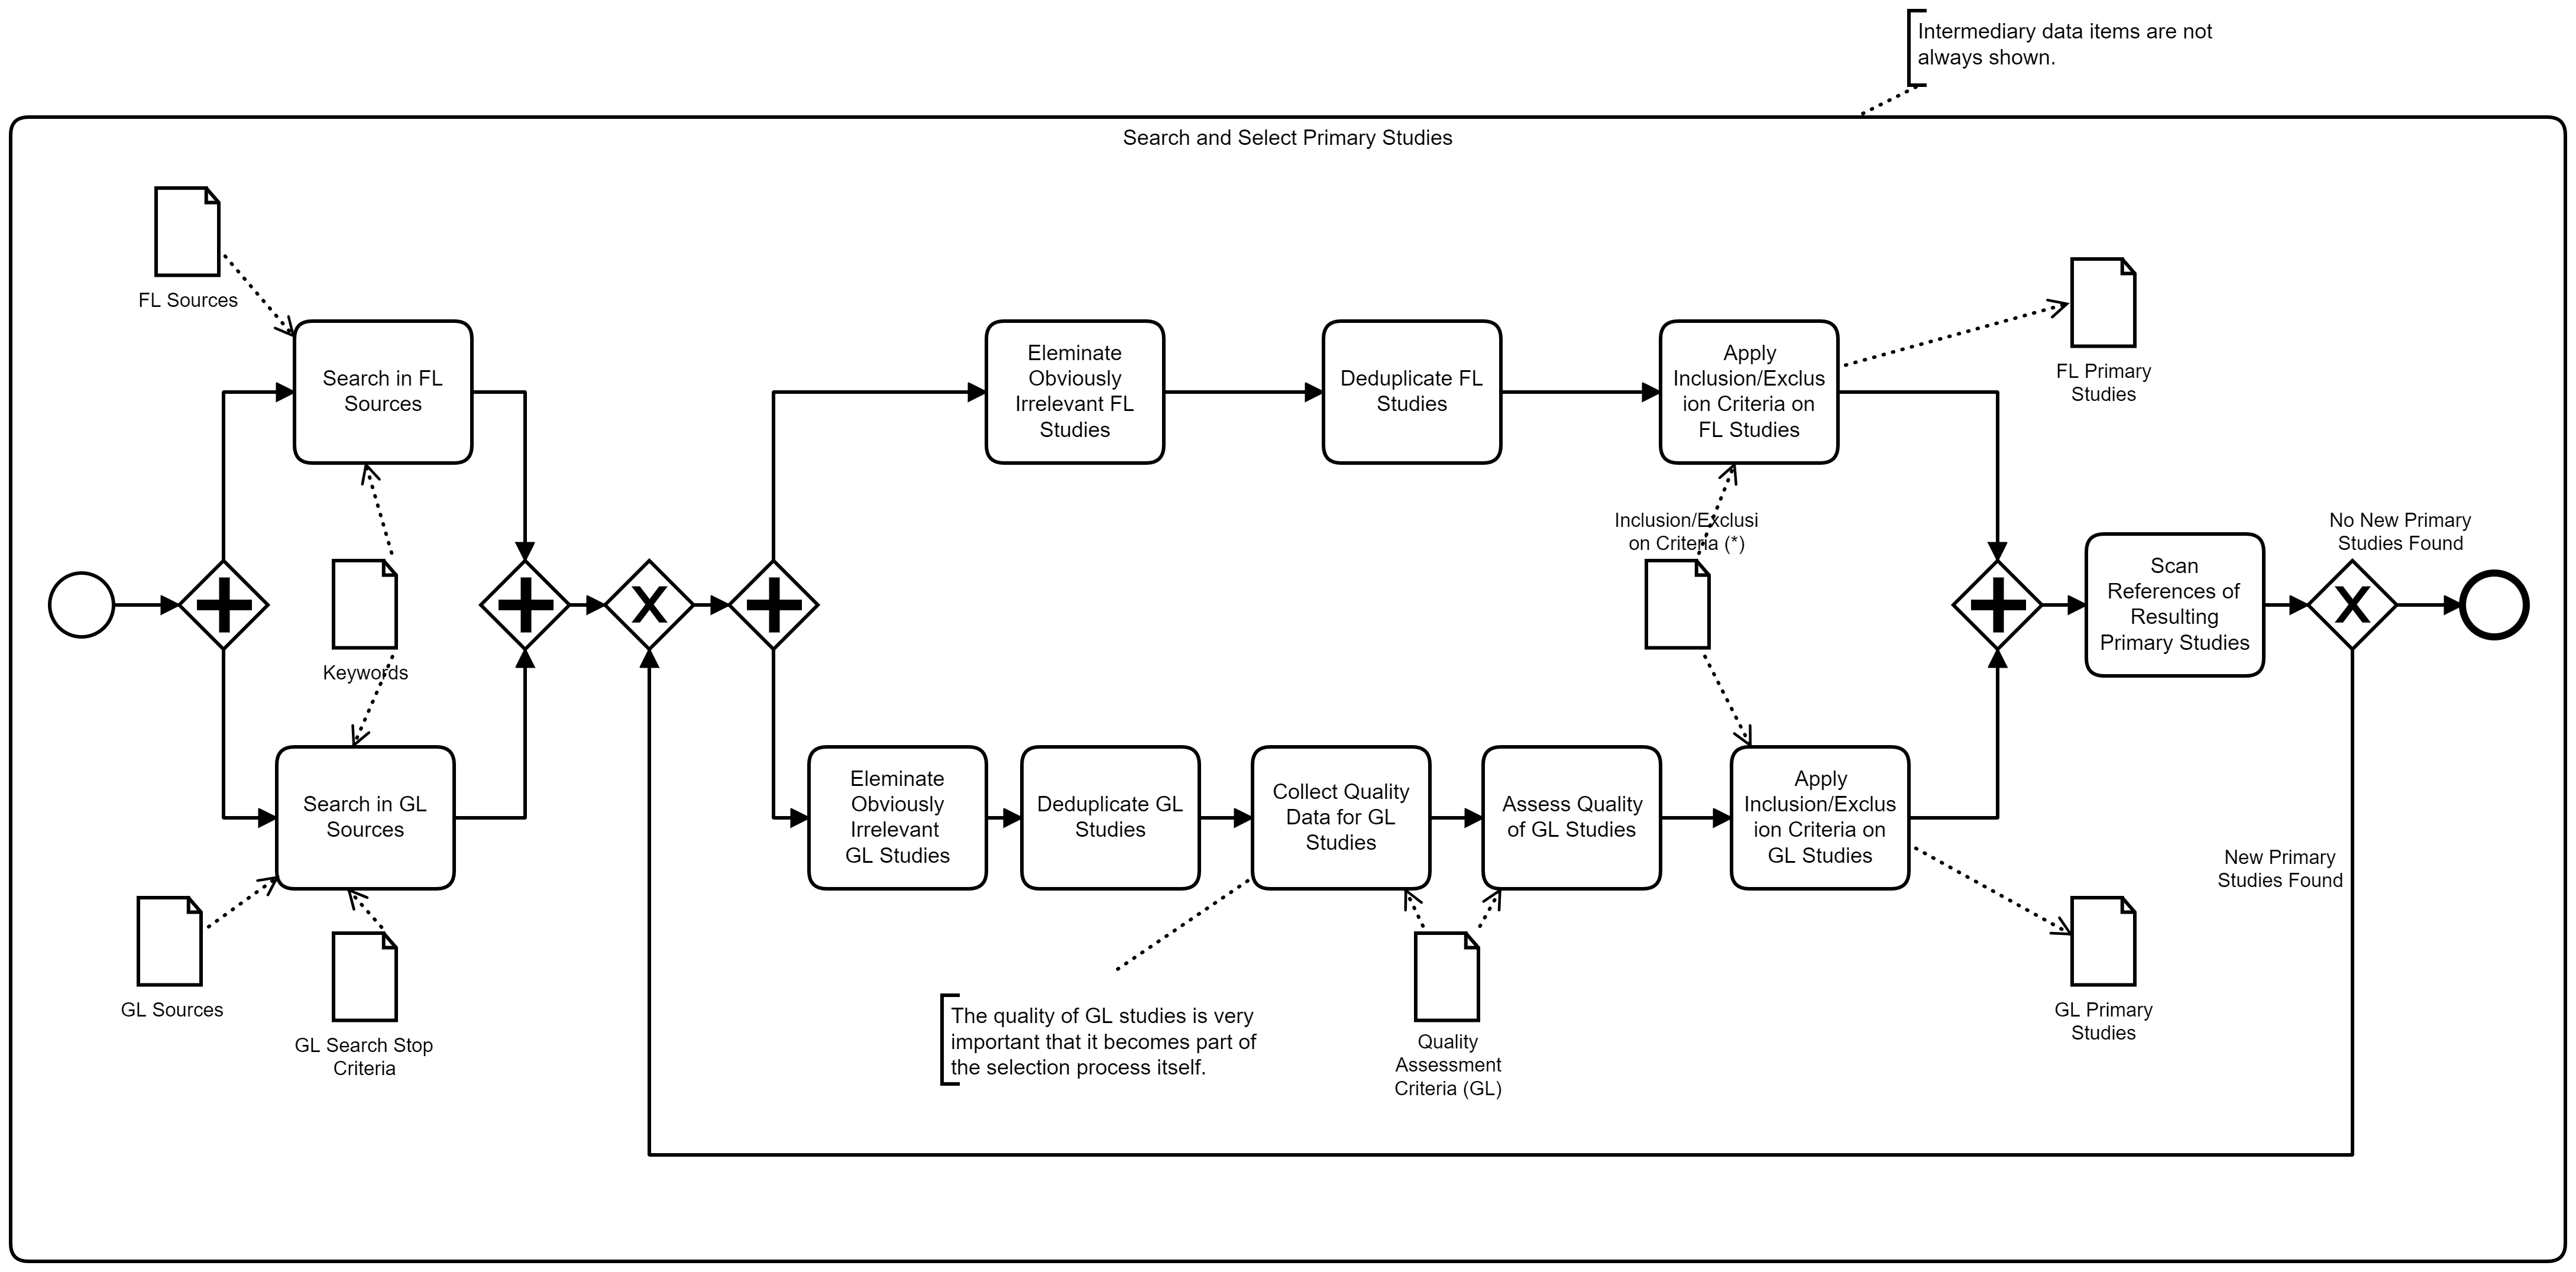
\includegraphics[width=\linewidth]{graphics/search-and-select}
			\caption[Search and select]{A detailed view of the steps to be taken during the activity of searching for and selecting the primary studies to be further analyzed.}
			\label{fig:search-and-select}
		\end{figure}
	\end{landscape}
}


\subsection{Source Selection}
\subsubsection{Formal Literature Sources}
We select a collection of diverse digital libraries that are known for publishing peer-reviewed (FL) articles related to computer science and that belong to scientific publishers.
These are:
\begin{inparaenum}[(i)]
	\item \href{https://dl.acm.org/}{ACM Digital Library},
	\item \href{https://ieeexplore.ieee.org/Xplore/home.jsp}{IEEE Xplore},
	\item \href{https://link.springer.com/}{SpringerLink},
	\item \href{https://www.sciencedirect.com/}{ScienceDirect}, and
	\item \href{https://onlinelibrary.wiley.com/}{Wiley Online Library}.
\end{inparaenum}

\subsubsection{Gray Literature Sources}
We select a collection of multidisciplinary preprint services for non-peer-reviewed scientific articles (GL) (we select all the services that have 500K+ articles accessible via their search interfaces\footnote{Estimated via the following Wikipedia article: \url{https://en.wikipedia.org/wiki/List_of_preprint_repositories} Visited on \today.}).
We also select Google Search as a general purpose search engine to find other kinds of GL items.
In total, the following sources are selected for GL studies:
\begin{inparaenum}[(i)]
	\item \href{https://osf.io/preprints/}{OSF Preprints},
	\item \href{https://papers.ssrn.com/sol3/DisplayAbstractSearch.cfm}{SSRN},
	\item \href{https://hal.archives-ouvertes.fr/}{HAL},
	\item \href{https://arxiv.org/}{arXiv}, and
	\item \href{https://google.com}{Google Search}.
\end{inparaenum}

Specifically, we will look for the following kinds of literature:
\begin{inparaenum}[(i)]
	\item Unpublished preprints,
	\item documentation of software systems,
	\item blog posts,
	\item theses for undergraduate or postgraduate degrees,
	\item white papers, and
	\item technical reports.
\end{inparaenum}
When searching in Google, we use the incognito mode of the browser to limit the effect of bias in ranking search results, which is influenced by the user's prior searches and interests.


\subsection{Search Query}
Due to the lack of standardization in the domain of blockchain interoperability, we try to include as many synonyms as possible for each unique term in the search query.
Furthermore, the concept of CCSCI is also not well established in the literature and thus lacks an agreed-upon name.
Therefore, we decided to make the search query rather permissive to increase the coverage at the expense of having a rather high rate of false positives.
We compensate for this with the inclusion and exclusion criteria to be applied in later steps.

We use the following query for the search:
\begin{lstlisting}[caption={The query term used to search for primary and secondary studies.},label={lst:query-string}]
	("inter?blockchain" | "cross?blockchain" | 
	"multi?blockchain" | "inter?chain" | "cross?chain" |
	"multi?chain" | "cross?ledger" | "multi?ledger" | 
	"inter?ledger" | "blockchain?interoperability" | 
	"ledger?interoperability" | "chain?interoperability") 
	& 
	(transaction | swap | invocation)
	&
	(blockchain | ledger)
	&
	("smart contract" | "chain?code")
\end{lstlisting}
The query is meant to be applied to the title, abstract, and keywords sections of each article (for articles), and for any part of the document (for non-article GL studies), and it serves as a template for the actual searches we will conduct.
This means that the exact query or queries applied will differ based on the specific sources.
As a rule of thumb, when the expressiveness of the search function of the source is limited, we choose a more permissive query, and apply filters on the outcomes to match the template query mentioned above.

We have tried this query on most selected sources, and in Google search yielding a reasonable number of results, with the first few looking closely related to the intended domain, which indicates a good balance between coverage and focus.

\subsection{Stopping Criteria}
We will perform exhaustive search when searching in \textit{digital libraries}, i.e., we will consider all results from applying the search query mentioned above.
However, in the case of Google, we will perform the search until theoretical saturation is reached~\cite{Garousi2017MLR}.
We consider that theoretical saturation is reached when \textit{20 consecutive search results do not introduce any new primary studies.}

\subsection{Deduplication}
Deduplication will be performed after merging the raw search results from the various sources.
The deduplication intended here is shallow to facilitate speed, i.e., it utilizes metadata about search results (title, authors, number of pages, type, date of publication, source), and not the actual content of the search result.
Therefore, it will not be able to detect two search results that refer to the same approach but with totally different titles.
Such duplicates will be discovered during the study selection process.
Here, two search results are considered as duplicates if the authors are the same, and the titles are either the same, or one indicates that it is an extended version of the other (usually has a similar title with the phrase "extended version" appended to it).
When a duplicate is found we follow the set of rules listed below in order until we have a match.
If no rule is matched, we select a random article from the two.

\begin{enumerate}
	\item If the full text of one article is accessible and the other is not, we select the accessible version.
	\item If one article is peer-reviewed (FL) and the other is not (GL), we select the peer-reviewed version.
	\item If both articles are not peer-reviewed, the one with higher source quality control is selected~\cite{Garousi2017MLR}.
	\item If one article is an extended version of the other, we select the extended version.
	\item If the articles have different dates, we select the newer version.
\end{enumerate}

\subsection{Snowballing}
Snowballing is the act of scanning the references used within a primary study to find new potential primary studies.
As shown in \Cref{fig:search-and-select}, we apply snowballing on the selected primary studies, i.e., primary studies that pass the inclusion and exclusion criteria.
Furthermore, the output of snowballing is fed back to the selection process (see \Cref{sec:study-selection-procedure}).

\section{Study Selection Criteria}
\label{sec:study-selection-criteria}
Here, we explain the inclusion and exclusion criteria for primary studies.
Certain criteria are unique to gray literature studies as shown below:

\subsection{Inclusion Criteria}
\begin{description}
	\item[IC1] The study language must be English.
	\item[IC2] The study must include a discussion of \textbf{own} blockchain interoperability approach\footnote{A blockchain interoperability approach must involve running business transactions that span resources on either (i) two or more blockchains, or (ii) one or more blockchains and one or more traditional software systems.} that enables CCSCIs.
\end{description}

\subsection{Exclusion Criteria}
\begin{description}
	\item[EC1] The primary objective of the study is not the discussion of own blockchain interoperability approach that enables or promises to enable CCSCIs. (e.g., secondary studies (reviews), studies discussing abstract concepts like paradigms or theorems rather than concrete approaches, or studies that don't enable CCSCIs \textcolor{red}{or that require large modifications in order to support CCSCIs} ).
	\item[EC2] Not enough details are provided about the approach.
	\item[EC3] (Deep deduplication) There is a more complete description of the same approach by a different primary study that has been selected~\footnote{This means that while progressing over search results, we might find a study that deselects previously selected studies because it is more complete than them. If an approach is not completely described by a single study, multiple studies can be selected to describe it.}.
	\item[EC4] If the study is GL, its \textit{inclusion score} must be achieved in full.
\end{description}

The \textit{inclusion score} of a GL study is defined as the sum of a subset of the quality criteria defined in \Cref{sec:study-quality-assessment}, that are deemed to be crucial.
Please refer to that section to find out which quality criteria constitute the inclusion score of GL studies.

\section{Study Selection Procedure}
\label{sec:study-selection-procedure}
The selection procedure goes through two steps as shown in \Cref{fig:search-and-select}.
First, search results that are obviously irrelevant are immediately excluded, then after shallow deduplication is performed, inclusion and exclusion criteria are carefully evaluated and applied, which includes calculating the quality score for GL studies.

\subsection{Initial Selection (Screening)}
In this step, search results that can be deemed irrelevant only based on the title, the abstract and the conclusion (evaluated in this order) are excluded.
This decision will not be documented, i.e., the reason will not be noted down.
Multiple researchers might perform screening on disjoint sets of search results independently without needing to verify each other's decisions.
Screening should be permissive, which means that if a study is not clearly irrelevant based on the title, the abstract and the conclusion, it must qualify for the detailed selection phase.

\subsection{Detailed Selection}
In this step, the full-text of each study is retrieved, and the inclusion and exclusion criteria are evaluated based on its contents.
For GL studies, if a study passes the inclusion criteria (IC1,IC2) and the exclusion criteria (EC1,EC2,EC3), its quality must be assessed before being selected (EC4).
To this end, certain data items are extracted from the study content and/or metadata (see \Cref{sec:study-quality-assessment}), and the quality score is calculated (see \Cref{sec:study-selection-criteria}).
If the quality score exceeds \textcolor{red}{XX}, the study is selected. 
Otherwise, it is not.
\textcolor{red}{Decisions at this stage are documented, and researchers must verify each other's decisions}.

\section{Study Quality Assessment}
\label{sec:study-quality-assessment}
We asses the quality of primary studies either to facilitate their selection process (in case of GL studies), or to facilitate ranking them (in case of FL studies).
We use a subset of the criteria proposed by Kitchenham et al.~\cite{Kitchenham2007SLR} for qualitative studies.
We also use a subset of the criteria proposed by Garousi et al.~\cite{Garousi2017MLR} for GL. 
\Cref{tab:quality-assessment} shows a summary of the chosen domain-independent study quality assessment criteria, and the possible values associated with each criterion.

\afterpage{%
	\begin{landscape}	
		\begin{table}[]
			\centering
			\caption{The criteria used to assess the quality of considered approaches. Criteria QC1-QC9 are applied to both GL and FL studies, whereas criteria QC10-QC16 are only applied to GL studies (assumed less relevant to FL studies)}
			\label{tab:quality-assessment}
			\begin{tabular}{l|l|l}
				\rowcolor[HTML]{EFEFEF} 
				ID & Quality Criterion & Possible Values \\ \hline
				QC1 & Is the goal clearly defined? & Yes (1) / No (0) \\
				QC2 & Is the approach described in detail? & Yes (1) / No (0) \\
				QC3 & How important/unique are the findings of the approach? & \begin{tabular}[c]{@{}l@{}}Important (1) / Important but not Unique (0.5) /\\ Not Important (0)\end{tabular} \\
				QC4 & Do the outcomes address the intended goal? & Yes (1) / No (0) \\
				QC5 & Is the link between the goal, the approach and the conclusion clear? & Yes (1) / Partially (0.5) / No (0) \\
				QC6 & Is a soundness proof of the approach included? & Yes (1) / No (0) \\
				QC7 & Can the approach be publicly validated (open-source implementation)? & Yes (1) / No (0) \\
				QC8 & Is the approach evaluated (scalability/performance/cost ...)? & Yes (1) / No (0) \\
				QC9 & Is the approach compared to other approaches? & Yes (1) / No (0) \\
				QC10 & Does the author / organization have expertise in the area? & Yes (1) / No (0) \\
				QC11 & Has the author / organization published other works in the field? & Yes (1) / No (0) \\
				QC12 & Are the approach limits clearly stated? & Yes (1) / Partially (0.5) / No (0) \\
				QC13 & Are the statements generally objective? & Yes (1) / Partially (0.5) / No (0) \\
				QC14 & Does the item have a clearly stated date? & Yes (1) / No (0) \\
				QC15 & Outlet type\cite{Garousi2017MLR} & \begin{tabular}[c]{@{}l@{}}1st tier GL (1)/ 2nd tier GL (0.5) /\\ 3rd tier GL (0)\end{tabular} \\
				QC16 & Is the project actively being maintained? (has activity in the last year) & Yes(1) / No(0)
			\end{tabular}
		\end{table}
	\end{landscape}
}

The inclusion score of GL studies (see \Cref{sec:study-selection-criteria}) includes the criteria QC1, QC2, QC7, and QC16.

\section{Data Extraction Strategy}
\label{sec:data-extraction-strategy}
The goal of this step is to collect the information needed to answer the research questions (see \Cref{sec:research-questions}), from the selected primary studies (see \Cref{sec:study-selection-procedure}).
To this end, data extraction forms are designed.
These forms include fields inferred from th research questions, in addition to some standard information such as the name of the reviewer, the date of the extraction, the metadata of the study, etc~\cite{Kitchenham2007SLR}.

\subsection{Data Extraction Forms}
\Cref{tab:data_extraction} shows the non-standard fields involved in the data extraction, which are meant to answer the research questions.
Note that RQ1 is answered via the search and selection procedures not by this form.
Furthermore, RQ6 is answered by a combination of this form and the quality assessment (see \Cref{sec:study-quality-assessment}).
\afterpage{%
	\begin{landscape}
		\begin{table}[ht]
			\centering
			\caption{The data extraction form for every selected primary study (not including standard fields).}
			\label{tab:data_extraction}
			\begin{tabular}{p{0.35\linewidth} | p{0.65\linewidth}}
				\rowcolor[HTML]{EFEFEF} 
				Data Item  &  Possible Values\\ \hline
				(RQ2) What are the steps involved in executing the CCSCI? & Textual description of how the CCSCI take place according to this approach. \\
				(RQ2) Who triggers the CCSCI? & The entity that triggers the execution of the CCSCI. Possible values could be: the end user, a smart contract, a validator, etc. \\
				(RQ2) Who manages the CCSCI? & The entity or entities that manage the execution of the CCSCI. Possible values could be: the end user, a smart contract, a validator, etc. \\
				(RQ2) What is the minimum number of end-users involved in the CCSCI? & The minimum number of end-users that must be involved in the execution of the CCSCI.\\
				(RQ3) What can be achieved with the CCSCI? & Textual description of the \textbf{documented} capabilities of the CCSCI approach.\\
				(RQ3) \textcolor{red}{What cannot be achieved?} & Textual description of the \textbf{documented} shortcomings of the CCSCI approach. \\
				(RQ3) Is the business transaction represented via the CCSCI predefined? & Yes / No \\
				(RQ4) What are the guarantees for honest participants? & One of the well-known transaction processing semantics, e.g., ACID, SAGA, or a textual description if new semantics are introduced. \\
				(RQ4) How is blockchain forking dealt with? & Text describing \textbf{if} blockchain forking is dealt witha and \textbf{how}.\\
				(RQ5) What types of blockchains are supported? & A list of supported blockchain systems (or types of systems). \\
				(RQ5) What types of non-blockchain systems are supported? & If the approach supports cross-domain CCSCIs, a list of supported non-blockchain systems is provided. \\
				(RQ5) Changes to existing systems & A list of changes to existing systems required to support the approach. \\
				(RQ6) \textcolor{red}{Is the approach implementation in production-ready state?} & Yes / No. 
			\end{tabular}
		\end{table}
\end{landscape}
}

\subsection{Data Extraction Procedure}
Studies are read carefully, and the information required to fill out the data extraction (and quality assessment forms for FL studies (see \Cref{sec:study-quality-assessment})) is extracted.
The researcher doing the extraction must maintain traceability~\cite{Garousi2017MLR}, i.e., the exact location from which every piece of extracted data is taken must be documented as a comment on the corresponding form.
It is planned that one researcher reads, extracts and fills out the forms, and another researcher verifies the entries by checking the traceability references.

\section{Synthesis of Extracted Data}
\label{sec:synthesis-of-extracted-data}
\textcolor{red}{Synthesis of extracted data is still an open question.}
Certain points to consider are:
\begin{list}{-}{}
	\item Certain data entries extracted from primary studies (see \Cref{sec:data-extraction-strategy}) are descriptive in nature.
	Therefore, we plan to apply qualitative data analysis techniques on such data entries to come up with meaningful categories (first cycle coding and pattern coding~\cite{Miles2014QualitativeDataAnalysis}).
	\item When coding phases are done, we plan to create a framework for comparing CCSCI approaches.
	\item We will present the extracted data after applying the comparison framework on it in a tabulated format.
	\item Statistics are generated based on the extracted data.
	\item Clear answers to the research questions are driven from the analyzed data.
\end{list}

\section{Dissemination Strategy}
\label{sec:dissemination-strategy}
TBD

\section{Timetable}
\label{sec:timetable}
TBD

\bibliography{bibliography,MasterBibliography}

\end{document}